\chapter{Parikshan}
\label{ch:parikshan}

\section{Introduction}
\label{sec:parikshanIntro}

Rapid resolution of incident (error/alert) management~\cite{sasase2013} in online service-oriented systems~\cite{microservice-book,hdfs,cassandra,redis} is extremely important.
The large scale of such systems means that any downtime has significant financial penalties for all parties involved.
However, the complexities of virtualized environments coupled with large distributed systems have made bug localization extremely difficult.
Debugging such production systems requires careful re-creation of a similar
environment and workload, so that developers can reproduce and identify the cause of the problem.

Existing state-of-art techniques for monitoring production systems rely on execution trace information. 
These traces can be replayed in a developer's environment, allowing them to use dynamic instrumentation and debugging tools to understand the fault that occurred in production.
On one extreme, these monitoring systems may capture only very minimal, high
level information, for instance, collecting existing log information and
building a model of the system and its irregularities from it~\cite{magpie,fay,failuresketching,problemsolvingSysTap}. \xxx{get more cites here too}
While these systems impose almost no overhead on the production system being
debugged (since they simply collect log information already being collected, or
have light-weight monitoring), they are limited in their fault finding and redproduction power, hence limited in their utility to developers.
On the other extreme, some monitoring systems capture complete execution traces, allowing the entire application execution to be exactly reproduced in a debugging environment \cite{odr,revirt,laadan2010transparent,geels2007friday}.
Despite much work towards minimizing the amount of such trace data captured, overheads imposed by such tracing can still be unacceptable for production use: in most cases, the overhead of tracing is at least 10\%, and it can balloon up to 2-10x overhead. \cite{pinplay,drdebug}.

We seek to allow developers to diagnose and resolve crashing and non-crashing failures of production service-oriented systems \emph{without suffering any performance overhead}.
Our key insight is that for most service-oriented systems, a failure can be reproduced simply by replaying the network inputs passed to the application.
For these failures, capturing very low-level sources of non-determinism (e.g. thread scheduling or general system calls, often with very high overhead) is unnecessary to successfully and automatically reproduce the buggy execution in a development environment.
We evaluated this insight by studying 16 real-world bugs (see Section~\ref{sec:parikshanCasestudy}), which we were able to trigger by only duplicating and replaying network packets.
Furthermore, we categorized 217 bugs from three real world applications, finding that most of these were similar in nature to the 16 that we reproduced. 
This suggests that our approach would be applicable to the bugs in our survey as well (see Section~\ref{sec:parikshanSurvey}).
%TODO - look into PRES to see if we can prove that capturing all sources of non-determinism is not important


Guided by this insight, we have created \parikshan\footnote{\parikshan is the \toolNameLang word for  testing}, which allows for real-time, online debugging of production services \textbf{\emph{without imposing any performance penalty}}.
At a high level, \parikshan leverages live cloning technology to create a sandboxed replica environment.
This replica is kept isolated from the real world so that developers can modify the running system in the sandbox to support their debugging efforts without fear of impacting the production system.
Once the replica is executing, \parikshan replicates all network inputs flowing to the production system, buffering and feeding them (without blocking the production system) to the debug system.
Within that debug system, developers are free to use heavy-weight instrumentation that would not be suitable in a production environment to diagnose the fault.
Meanwhile, the production system can continue to service other requests.
\parikshan can be seen as very similar to tools such as Aftersight \cite{aftersight} that offload dynamic analysis tasks to replicas and VARAN \cite{Hosek:2015:VUE:2694344.2694390} that support multi-version execution, but differs in that its high-level recording level (network inputs, rather than system calls) allows it to have significantly lower overhead.


%\parikshan primarily focuses on bugs~\cite{Zhang:2013:ADS:2486788.2486830, liu2005mining, kremenek2007factor}.
\parikshan focuses on helping developers debug faults \emph{online} --- as they occur in production systems.
We expect \parikshan to be used in cases of tricky bugs that are highly sensitive to their environment, such as semantic bugs, performance bugs, resource-leak errors, configuration bugs, and concurrency bugs.
Although in principle, \parikshan can be used to diagnose crashing bugs, we target primarily non-crashing bugs, where it is important for the production system to remain running even after a bug is triggered, for instance, to continue to process other requests. 
%For instance, semantic bugs are caused because of logical errors, which lead to an unexpected output, performance bugs result in a slow-down of the application. 
We present a more detailed explanation of these categories in Section~\ref{sec:parikshanCasestudy}.

%We assume our target system has been deployed based on micro-service architecture~\cite{microservice-book,microservices}, which advocates running each service in isolation.
We leverage container virtualization technology (e.g., Docker~\cite{docker}, OpenVZ~\cite{openvz}), which can be used to pre-package services so as to make deployment of complex multi-tier systems easier (i.e. DockerHub~\cite{dockerhub,dockerhub_article} provides pre-packaged containers for storage, webserver, database services etc.).
Container based virtualization is now increasingly being used in practice~\cite{containerCloud}.
In contrast to VM's containers run natively on the physical host (i.e. there is no hypervisor layer in between), this means that there is no additional overhead, and near-native performance for containers~\cite{performanceComparisonlxcVM,performanceEvalContainers}.
While \parikshan could also be deployed using VM's, container virtualization is much more light weight in terms of resource usage.

%Essentially, micro-service architecture allows us to launch debug containers which targets one service at a time. 
%This is not a necessary condition, but makes deploying \parikshan easier and more practical.

%We leverage user-space container virtualization technologies (OpenVZ/LXC~\cite{openvz,lxc}).
%For simplicity, we assume that our target systems utilize service-oriented architectures, where each service (application, DNS, indexing, storage) is sandboxed in separate containers (\texttt{OpenVZ}~\cite{openvz}).
%This allows us to launch debug containers, which can target one application component at a time.
%While our techniques can also be applied to traditional VMs, containers are lighter-weight and use far fewer resources.

\noindent
The key benefits of our system are:
\begin{itemize}[leftmargin=*,topsep=0pt,itemsep=-1ex,partopsep=1ex,parsep=1ex]
\item \textbf{Zero Overhead Monitoring:} While existing approaches have focused on minimizing the recording overhead. 
\parikshan uses novel non-blocking network duplication to avoid any overhead at all in the production environment.	
\item \textbf{Sandbox debugging:} \parikshan provides a cloned sandbox environment to debug the production application.
This allows a safe mechanism to diagnose the error, without impacting the functionality of the application.
\item \textbf{Capture large-scale context:} Allows capturing the context of large scale production systems, with long running applications. Under normal circumstances capturing such states is extremely difficult as they need a long running test input and large test-clusters.
%\item \textbf{Short time-to-debug:} These techniques contribute to a shortened debug time, by allowing debuggers to directly gather trace data, without needing to bring down the system. 
\end{itemize}

\noindent
The rest of the paper is organized as follows.
Section~\ref{sec:parikshanDesign} and \ref{sec:parikshanImplementation} describe the design and implementation of \parikshan and each of it's internal components.
We then present a case study of 16 real-world bugs successfully reproduced by \parikshan in Section~\ref{sec:parikshanCasestudy}.
%We have tested \parikshan live network duplication process to re-create 16 production bugs in 5 well-known software systems (MySQL, Apache HTTPD, Redis, Hadoop/HDFS) see section~\ref{sec:casestudy}. 
%Furthermore, we performed a survey of Bugzilla reports of apache and MySQL to show that a majority of bugs in production systems can be classified in 5 categories that can in principle be handled by \parikshan (see section~\ref{sec:survey}).
This is followed by the evaluation in Section~\ref{sec:parikshanEvaluation}.
In Section~\ref{sec:parikshanApplication}, we discuss potential applications of \parikshan. 
Finally, we discuss some challenges in Section~\ref{sec:parikshanThreats} and conclude.


\begin{figure*}[t]
	\begin{centering}
		\includegraphics[width=0.99\textwidth]{parikshan/figs/arch_full.pdf}
		\caption{\textbf{High level architecture of \parikshan}, showing the main components: Network Duplicator, Network Aggregator, and Cloning Manager. The replica (debug container) is kept in sync with the master (production container) through network-level record and replay. In our evaluation, we found that this light-weight procedure was sufficient to reproduce many real bugs.}
		\label{fig:network_arch}
	\end{centering}
\end{figure*}



\section{\parikshan}
\label{sec:parikshanDesign}

In Figure~\ref{fig:network_arch}, we show the architecture of \parikshan when applied to a single mid-tier application server.
\parikshan consists of 3 modules: 
\textbf{Clone Manager}: manages ``live cloning'' between the production containers and the debug replicas, 
\textbf{Network Duplicator}: manages network traffic duplication from downstream servers to both the production and debug containers, 
and \textbf{Network Aggregator}: manages network communication from the production and debug containers to upstream servers.
The network duplicator also performs the important task of ensuring that the production and debug container executions do not diverge.
The duplicator and aggregator can be used to target multiple connected tiers of a system by duplicating traffic at the beginning and end of a workflow.
Furthermore, the aggregator module is not required if the debug-container has no upstream services. 
%At the end of this section, we also discuss the \textbf{debug window} during which we believe that the debug-container faithfully represents the execution of the production container.
%Finally, we discuss \textbf{divergence checking} which allows us to observe if the production and debug containers are still in sync.



\begin{figure}[ht]
	\begin{center}
		\includegraphics[width=0.9\textwidth]{parikshan/figs/ModesCloning.pdf}
		\caption{External and Internal Mode for live cloning: P1 is the production, and D1 is the debug container, the clone manager interacts with an agent which has drivers to implement live cloning.}
		\label{fig:modesCloning}
	\end{center}
\end{figure}


\subsection{Clone Manager} 
\label{sec:parikshanCloneManager}

Live migration~\cite{mirkin2008containers,clark2005live,gebhart2009dynamic} refers to the process of moving a running virtual machine or container from one server to another, without disconnecting any client or process running within the machine (this usually incurs a short or negligible suspend time). 
In contrast to live migration where the original container is destroyed, the ``Live Cloning'' process used in \parikshan requires both containers to be actively running, and be still attached to the original network.
The challenge here is to manage two containers with the same identities in the network and application domain. 
This is important, as the operating system and the application processes running in it may be configured with IP addresses, which cannot be changed on the fly.
Hence, the same network identifier should map to two separate addresses, and enable communication with no problems or slowdowns.

\noindent
We now describe two modes (see Figure~\ref{fig:modesCloning}) in which cloning has been applied, followed by the algorithm for live cloning:

\begin{itemize}
	
	\item \textbf{\textit{Internal Mode}}: In this mode, we allocate the production and debug containers to the same host node. 
	This would mean less suspend time, as the production container can be locally cloned (instead of streaming over the network). 
	Additionally, it is more cost-effective since the number of servers remain the same.
	On the other hand, co-hosting the debug and production containers could potentially have an adverse effect on the performance of the production container because of resource contention.
	Network identities in this mode are managed by encapsulating each container in separate network namespaces~\cite{netns}.
	This allows both containers to have the same IP address with different interfaces.
	The duplicator is then able to communicate to both these containers with no networking conflict.
	
	
	\item \textbf{\textit{External Mode}}: In this mode we provision an extra server as the host of our debug-container (this server can host more than one debug-container). 
	While this mechanism can have a higher overhead in terms of suspend time (dependent on workload) and requires provisioning an extra host-node, the advantage of this mechanism is that once cloned, the debug-container is totally separate and will not impact the performance of the production-container.
	We believe that external mode will be more practical in comparison to internal mode, as cloning is likely to be transient, and high network bandwidth between physical hosts can offset the slowdown in cloning performance. 
	Network identities in external mode are managed using NAT~\cite{nat} (network address translator) in both host machines. 
	Hence both containers can have the same address without any conflict.\footnote{Another additional mode can be \textit{Scaled Mode}: This can be viewed as a variant of the external mode, where we can execute debug analysis in parallel on more than one debug-containers each having its own cloned connection. This will distribute the instrumentation load and allow us to do more analysis concurrently, without overflowing the buffer. We aim to explore this in the future.}
	
\end{itemize}

Algorithm \ref{algCloning} describes the specific process for cloning some production container P1 from Host H1 to replica D1 on Host H2.


\begin{algorithm}[ht!]
	\caption{Live cloning algorithm using OpenVZ} 
	\label{algCloning}
	\begin{enumerate}[topsep=0pt,itemsep=-1ex,partopsep=1ex,parsep=1ex]
		\item Safety checks and pre-processing (ssh-copy-id operation for password-less rsync, checking pre-existing container ID's, version number etc.) 
		\item Create and synchronize file system of P1 to D1  
		\item Set up port forwarding, duplicator, and aggregator
		\item Suspend the production container P1
		\item Checkpoint \& dump the process state of P1
		\item Since step 2 and 5 are non-atomic operations, some files may be outdated.
		A second sync is run when the container is suspended to ensure P1 and D1 have the same state
		\item Resume both production and debug containers
	\end{enumerate}
\end{algorithm}


The suspend time of cloning depends on the operations happening within the container between step 2 and step 4 (the first and the second rsync), as this will increase the number of dirty pages in the memory, which in turn will impact the amount of memory that needs to be copied during the suspend phase.
This suspend time can be viewed as an amortized cost in lieu of instrumentation overhead.
We evaluate the performance of live cloning in Section~\ref{sec:parikshanPerformance}.

\subsection{Network Proxy Design Description}

The network proxy duplicator and aggregator are composed of the following internal components:

\begin{itemize}[leftmargin=*]
	\item \textbf{Synchronous Passthrough}: The synchronous passthrough is a daemon that takes the input from a source port, and forwards it to a destination port. The passthrough is used for communication from the production container out to other components (which is not duplicated).
	\item \textbf{Asynchronous Forwarder}: The asynchronous forwarder is a daemon that takes the input from a source port, and forwards it to a destination port, and also to an internal buffer. The forwarding to the buffer is done in a non-blocking manner, so as to not block the network forwarding. 
	\item \textbf{Buffer Manager}: Manages a FIFO queue for data kept internally in the proxy for the debug-container.
	It records the incoming data, and forwards it a destination port. 
	\item \textbf{Dummy Reader}: This is a standalone daemon, which reads and drops packets from a source port
\end{itemize}

\noindent
%Next, we explain how these components are used:\\



\iffalse
\begin{figure}[ht]
	\begin{centering}
		\includegraphics[width=0.9\textwidth]{parikshan/figs/network_dup.pdf}
		%    \captionsetup{justification=centering}
		\caption{Network Duplicator: Thread 1 sends traffic on links 1 and 3, Thread 2 manages links 2 and 4, Thread 3 forwards traffic on link 5, \& Thread 4 reads and drops data on link 6}
		\label{fig:duplicator}
	\end{centering}
\end{figure}
\fi



\subsubsection{Proxy Network Duplicator:} 
\label{sec:parikshanProxyDuplicator}
To successfully perform online debugging in the replica to work, both production and debug containers must receive the same input.
A major challenge in this process is that the production and debug container may execute at different speeds (debug will be slower than production): this will result in them being out of sync.
Additionally, we need to accept responses from both servers and drop all the traffic coming from the debug-container, while still maintaining an active connection with the client.
Hence simple port-mirroring and proxy mechanisms will not work for us. 

TCP is a connection-oriented protocol and is designed for stateful delivery and acknowledgment that each packet has been delivered.
Packet sending and receiving are blocking operations, and if either the sender or the receiver is faster than the other the send/receive operations are automatically blocked or throttled.
This can be viewed as follows: Let us assume that the client was sending packets at $X Mbps$ (link 1), and the production container was receiving/processing packets at $Y Mbps$ (link 2), where $Y<X$. 
Then automatically, the speed of link 1 and link 2 will be throttled to $Y Mbps$ per second, i.e the packet sending at the client will be throttled to accommodate the production server. 
Network throttling is a default TCP behavior to keep the sender and receiver synchronized.
However, if we also send packets to the debug-container sequentially in link 3 the performance of the production container will be dependent on the debug-container. 
If the speed of link 3 is $Z$ $Mbps$, where $Z < Y$, and $Z < X$, then the speed of link 1, and link 2 will also be throttled to $Z$ $Mbps$.
The speed of the debug container is likely to be slower than production: this may impact the performance of the production container.

Our solution is a customized TCP level proxy. 
This proxy duplicates network traffic to the debug container while maintaining the TCP session and state with the production container. 
Since it works at the TCP/IP layer, the applications are completely oblivious to it.
To understand this better let us look at Figure~\ref{fig:network_arch}: Here each incoming connection is forwarded to both the production container and the debug container . 
This is a multi-process job involving 4 parallel processes (P1-P4): In P1, the asynchronous forwarder sends data from client to the production service, while simultaneously sending it to the buffer manager in a non-blocking send.  This ensures that there is no delay in the flow to the production container because of slow-down in the debug-container.
In P2, the pass-through forwarder reads data from the production and sends it to the client (downstream component).
Process P3, then sends data from Buffer Manager to the debug container, and Process P4 uses a dummy reader, to read from the production container and drops all the packets

\iffalse
To avoid a slowdown in the production container, we use 4 threads T1, T2, T3, T4  to manage each incoming connection to the proxy.
Thread T1 forwards packets from the client to the proxy (link 1), and from the proxy to the production container (link 3). 
It then uses a non-blocking send to forward packets to an internal pipe buffer shared between thread T1, and thread T3.
Thread T2 reads the responses from the production container and forwards them to the client (link 4 and 2).
Thread T3 then reads from this piped buffer and sends the  traffic forward to the debug-container( link 5), while Thread T4, receives packets from the debug-container and drops them (link 6).
\fi

The above strategy allows for non-blocking packet forwarding and enables a key feature of \parikshan, whereby it avoids slowdowns in the debug-container to impact the production container.
We take the advantage of an in-memory buffer, which can hold requests for the debug-container, while the production container continues processing as normal.
A side-effect of this strategy is that if the speed of the debug-container is too slow compared to the packet arrival rate in the buffer, it may eventually lead to an overflow. 
We call the time taken by a connection before which the buffer overflows its \emph{debug-window}.
We discuss the implications of the \emph{debug window} in Section \ref{sec:parikshanWindow}.  

\iffalse
\begin{figure}[ht!]
	\begin{center}
		\includegraphics[width=0.9\textwidth]{parikshan/figs/aggregator.pdf}
		%    \captionsetup{justification=centering}
		\caption{Description of the Network Aggregator. Thread 1 executes step [1,3], Thread 2 step [2,4], and Thread 3 step [5], and Thread 4 step [6]}
		\label{fig:aggregator}
	\end{center}
\end{figure}
\fi


\subsubsection{Proxy Network Aggregator:}
\label{sec:parikshanProxyAggregator}
The proxy described in Section~\ref{sec:parikshanProxyDuplicator} is used to forward requests from downstream tiers to production and debug containers.
While the network duplicator duplicates incoming requests, the network aggregator manages incoming ``responses'' for requests sent from the debug container. 
Imagine if you are trying to debug a mid-tier application container, the proxy network duplicator will replicate all incoming traffic from the client to both debug and the production container. 
Both the debug container and the production, will then try to communicate further to the backend containers.
This means duplicate queries to backend servers (for instance, sending duplicate `delete' messages to MySQL), thereby leading to an inconsistent state.
Nevertheless, to have forward progress the debug-container must be able to communicate and get responses from upstream servers.
The ``proxy aggregator'' module stubs the requests from a duplicate debug container by replaying the responses sent to the production container to the debug-container and dropping all packets sent from it to upstream servers.

As shown in  Figure~\ref{fig:network_arch}, when an incoming request comes to the aggregator, it first checks if the connection is from the production container or debug container. 
In process P1, the aggregator forwards the packets to the upstream component using the pass-through forwarder.
In P2, the asynchronous forwarder sends the responses from the upstream component to the production container, and sends the response in a non-blocking manner to the internal queue in the buffer manager. 
Once again this ensures no slow-down in the responses sent to the production container.
The buffer manager then forwards the responses to the debug container (Process P3).
Finally, in process P4 a dummy reader reads all the responses from the debug container and discards them.

%Responses from the backend server are sent to the aggregator (link 4), and then forwarded to the production container (link 2) and simultaneously saved in an internal queue.
%The aggregator creates an in-memory persistent inter-process FIFO queue for each connection where the responses for each of these connections are stored.
%When the corresponding connection from the duplicate debug container connects to the proxy (link 5); all packets being sent are quietly dropped. 
%The aggregator then uses the queue to send replies to the debug-container (link 6).
%In a way this is a streaming online record-and-replay, where we are recording the data in our buffer.

We assume that the production and the debug container are in the same state, and are sending the same requests. 
Hence, sending the corresponding responses from the FIFO queue instead of the backend ensures:
(a) all communications to and from the debug container are isolated from the rest of the network,
(b) the debug container gets a logical response for all it's outgoing requests, making forward progress possible,
and (c). similar to the proxy duplicator, the communications from the proxy to internal buffer is non-blocking to ensure no overhead on the production-container.

%In this design we assume that the order of incoming connections remains largely the same.
%To allow for some flexibility, we use a fuzzy checking mechanism using the hash value of the da%ta being sent to correlate the connections. 
%Each queue has a short wait time to check against incoming connections, this allows us to match slightly out of order connections.
%In case a connection cannot be correlated, we send a TCP\_FIN, to close the connection, and inform the user.
%\xxx{Does this come up? Need to talk about that as a limitation if so, or give some evidence that it doesnt otherwise}
%\yyy{you are right removed, actually I needed to update the network aggregator anyways}
%In case a connection cannot be correlated, we allow the connection to time out and send a TCP\_FIN.


\subsection{Debug Window}
\label{sec:parikshanWindow}

\parikshan's asynchronous forwarder uses an internal buffer to ensure that incoming requests proceed directly to the production container without any latency, regardless of the speed at which the debug replica processes requests.
The incoming request rate to the buffer is dependent on the user, and is limited by how fast the production container manages the requests (i.e. the production container is the rate-limiter).
The outgoing rate from the buffer is dependent on how fast the debug-container processes the requests.
Instrumentation overhead in the debug-container can potentially cause an increase in the transaction processing times in the debug-container.
As the instrumentation overhead increases, the incoming rate of requests may eventually exceed the transaction processing rate in the debug container.
If the debug container does not catch up, this in turn can lead to a buffer overflow. We call the time period until buffer overflow happens the \emph{debug-window}.
This depends on the size of the buffer, the incoming request rate, and the overhead induced in the debug-container. 
For the duration of the debugging-window, we assume that the debug-container faithfully represents the production container. 
Once the buffer has overflown, the debug-container may be out of sync with the production container. 
At this stage, the production container needs to be re-cloned, so that the replica is back in sync with the production and the buffer can be discarded.
In case of frequent buffer-overflows, the buffer size needs to be increased or the instrumentation to be decreased in the replica, to allow for longer debug-windows.

The debug window size also depends on the application behavior, in particular how it launches TCP connections. 
\parikshan generates a pipe buffer for each TCP connect call, and the number of pipes are limited to the maximum number of connections allowed in the application.
Hence, buffer overflows happen only if the requests being sent in the same connection overflow the queue.
For webservers, and application servers, the debugging window size is generally not a problem, as each request is a new ``connection.''
This enables \parikshan to tolerate significant instrumentation overhead without a buffer overflow.
On the other hand, database and other session based services usually have small request sizes, but multiple requests can be sent in one session which is initiated by a user. 
In such cases, for a server receiving a heavy workload, the number of calls in a single session may eventually have a cumulative effect and cause overflows.

To further increase the \emph{debug window}, we propose load balancing debugging instrumentation overhead across multiple debug-containers, which can each get a duplicate copy of the incoming data. 
For instance, debug-container 1 could have 50\% of the instrumentation, and the rest on debug-container 2.
We believe such a strategy would significantly reduce the chance of a buffer overflow in cases where heavy instrumentation is needed.
Section~\ref{sec:parikshanTimewindowPerformance} explains in detail the behavior of the debug window, and how it is impacted by instrumentation.
\xxx{What happens when we exceed the debug window?}


\subsection{Divergence Checking}
\label{sec:parikshanDivergenceChecking}

In \parikshan it is possible that non-deterministic behavior (discussed in Section~\ref{sec:parikshanThreatsNonDeterminism}) in the two containers or user instrumentation, causes the production and debug container to diverge with time.
To understand and capture this divergence, we compare the corresponding network output received in the proxy.
This is an optional component, which gives us a black-box mechanism to check the fidelity of the replica based on its communication with external components.
In our current prototype, we use a hash on each data packet, which is collected and stored in memory for the duration that each packet's connection is active.
The degree of acceptable divergence is dependent on the application behavior, and the operator's wishes. 
For example, an application that includes timestamps in each of its messages (i.e. is expected to have some non-determinism) could perhaps be expected to have a much higher degree of acceptable divergence than an application that should normally be returning deterministic results.



\subsection{Implementation}
\label{sec:parikshanImplementation}
%\xxx{I feel like maybe this section is describing the evaluation environment. In which case, we need to talk about that in such a context, and still say something about implementation}
%\xxx{Where is the architecture diagram? The system diagram? What did we build? What are the modules? How do they talk to each other? What are the system requirements? Does it *only* run on Nipun's specially configured laptop?}
%\xxx{We are talking about kernel version why? Does the implemetation have anything to do with hacking on the kernel? The distro? Why are we going on about it?}
The clone-manager and the live cloning utility are built on top of the user-space container virtualization software OpenVZ~\cite{openvz}.
\parikshan extends \emph{VZCTL} 4.8~\cite{vzctl} live migration facility~\cite{mirkin2008containers}, to provide support for online cloning.
To make \textbf{live cloning} easier and faster, we used OpenVZ's \textit{ploop} devices~\cite{ploop} as the container disk layout.
The network isolation for the production container was done using Linux network namespaces~\cite{netns} and NAT~\cite{nat}.
While \parikshan is based on light-weight containers, we believe that \parikshan can easily be applied to heavier-weight, traditional virtualization software where live migration has been further optimized~\cite{liveVMprinciples,trafficliveVM}.
%The reason for choosing a container based implementation was that containers take much less resources in comparison to traditional VM's.

The network proxy duplicator and the network aggregator was implemented in C/C++.
The forwarding in the proxy is done by forking off multiple processes each handling one send/or receive a connection in a loop from a source port to a destination port.
Data from processes handling communication with the production container, is transferred to those handling communication with the debug containers using \emph{Linux Pipes}~\cite{linuxpipes}.
Pipe buffer size is a configurable input based on user-specifications.


\section{Evaluation}
\label{sec:parikshanEvaluation}

To evaluate the performance of \parikshan, we pose and answer the following research questions:

\begin{itemize}
\item \textbf{RQ1:} How long does it take to create a live clone of a production container and what is it's impact on the performance of the production container?\\
\item \textbf{RQ2:} What is the size of the debugging window, and how does it depend on resource constraints?\\ 
\item \textbf{RQ3:} Can we generalize the results of our case study to see if \parikshan can target even more real bugs?
\end{itemize}

We evaluated the \textbf{internal mode} on two identical VM's with an Intel i7 CPU, with 4 Cores, and 16GB RAM each in the same physical host (one each for production and debug containers).
We evaluated the \textbf{external mode} on two identical host nodes with Intel Core 2 Duo Processor, 8GB of RAM.
All evaluations were performed on CentOS 6.5.

%In Section~\ref{sec:performance}, we evaluate live cloning on real-world applications and workloads as well as a micro-benchmark to understand its performance in different scenarios.
%In Section~\ref{sec:timewindowPerformance}, we first provide debug-window sizes for varying workloads run on a live production system. 
%For a more systematic understanding of the debug-window size, we also provide simulation results to show the relationship of buffer overflow with buffer size, the incoming workload, and the instrumentation overhead.
%Finally, in Section~\ref{sec:survey}, we present a survey of 217 real-world bugs, picked from three different applications.
%\xxx{What is the environment we evaluated in? Hardware? Software? Why do we have both real and simulated data?}

\subsection{Live Cloning Performance}
\label{sec:parikshanPerformance}

As explained in Section \ref{sec:design}, a short suspend time during live cloning is necessary to ensure that both containers are in the exact same system state.
The suspend time during live cloning can be divided in 4 parts: 
(1) Suspend \& Dump: time taken to pause and dump the container, 
(2) Pcopy after suspend: time required to complete rsync operation 
(3) Copy Dump File: time taken to copy an initial dump file.
(4) Undump \& Resume: time taken to resume the containers. 
To evaluate ``live cloning'', we ran a micro-benchmark of I/O operations, and evaluated live-cloning on some real-world applications running real-workloads.

\begin{figure}[ht]
  \centering
  \resizebox{.8\linewidth}{!}{
    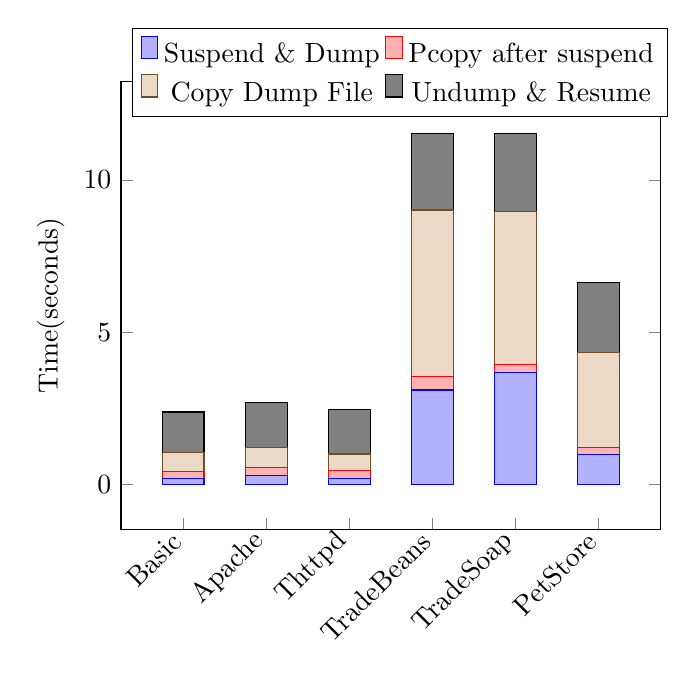
\begin{tikzpicture}
      \begin{axis}[
        ybar stacked,
        bar width=15pt,
        %	nodes near coords,
        enlargelimits=0.15,
        legend style={at={(0.02,1.12)},anchor=north west,legend columns=2},
        ylabel={Time(seconds)},
        symbolic x coords={Basic, Apache, Thttpd, TradeBeans, TradeSoap, 
          PetStore},
        xtick=data,
        x tick label style={rotate=45,anchor=east},
        ]
        \addplot+[ybar] plot coordinates {(Basic,0.21) (Apache,0.30) (Thttpd,0.21) (TradeBeans,3.10) (TradeSoap,3.68) (PetStore,0.97) };
        \addplot+[ybar] plot coordinates {(Basic,0.22) (Apache,0.27) (Thttpd,0.26) (TradeBeans,0.44) (TradeSoap,0.25) (PetStore,0.24) };
        \addplot+[ybar] plot coordinates {(Basic,0.62) (Apache,0.64) (Thttpd,0.53) (TradeBeans,5.47) (TradeSoap,5.03) (PetStore,3.11) };
        \addplot+[ybar] plot coordinates {(Basic,1.33) (Apache,1.47) (Thttpd,1.46) (TradeBeans,2.51) (TradeSoap,2.57) (PetStore,2.32) };
        \addlegendentry{\strut Suspend \& Dump}
        \addlegendentry{\strut Pcopy after suspend}
        \addlegendentry{\strut Copy Dump File}
        \addlegendentry{\strut Undump \& Resume}
      \end{axis}
    \end{tikzpicture}
   }
  %\captionsetup{justification=centering}
  \caption{Suspend time for live cloning, when running a representative benchmark}
  \label{fig:stats}
\end{figure}


\subsubsection{Real world applications and workloads:}
To begin to study the overhead of live cloning, we performed an evaluation using five well-known applications.
Figure~\ref{fig:stats} presents the suspended times for five well-known applications when cloning a replica with \parikshan. 
We ran the httperf~\cite{httperf} benchmark on Apache and \emph{thttpd} to compute max throughput of the web-servers, by sending a large number of concurrent requests.
Tradebeans and Tradesoap are both part of the dacapo~\cite{dacapo} benchmark ``DayTrader'' application.
These are realistic workloads, which run on a multi-tier trading application provided by IBM. 
PetStore~\cite{petstore} is also a well known J2EE reference application. 
We deployed PetStore in a 3-tier system with JBoss, MySQL and Apache servers, and cloned the app-server.
The input workload was a random set of transactions which were repeated for the duration of the cloning process.

As shown in Figure~\ref{fig:stats}, for Apache and Thttpd the container suspend time ranged between 2-3 seconds.
However, in more memory intensive application servers such as PetStore and DayTrader, the total suspend time was higher (6-12 seconds).
Nevertheless, we did not experience any timeouts or errors for the requests in the workload\footnote{In case of packet drops, requests are resent both at the TCP layer, and the application layer. This slows down the requests for the user, but does not drop them}.
However, this did slowdown requests in the workload. 
This shows that short suspend times are largely not visible or have minimal performance impact to the user, as they are within the time out range of most applications.
Further, a clean network migration process ensures that connections are not dropped, and are executed successfully.
We felt that these relatively fast temporary app suspensions were a reasonable price to pay to launch an otherwise overhead-free debug replica.
To further characterize the suspend time imposed by the live cloning phase of \parikshan, we created a synthetic micro-benchmark to push \parikshan towards its limit.
\begin{figure}[ht]
%{0.45\textwidth}
  \centering
  \resizebox{.8\linewidth}{!}{
%\begin{adjustbox}{max size={.9\textwidth}}
    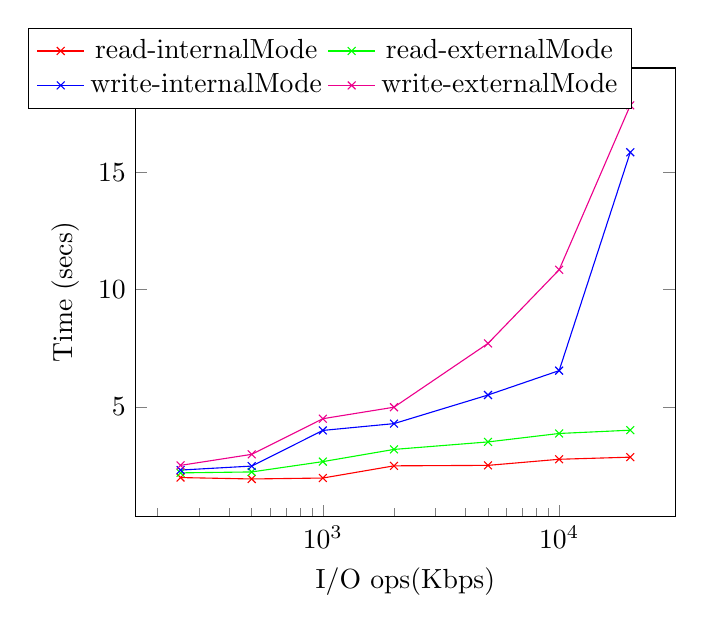
\begin{tikzpicture}
      \begin{axis}[
        xmode=log,
        legend style={at={(-0.2,1.09)},anchor=north west,legend columns=2},
        xlabel=I/O ops(Kbps),
        ylabel=Time (secs)]
        \addplot[color=red,mark=x] coordinates {
          (0,1.85)
          (250,1.99)
          (500,1.93)
          (1000,1.97)
          (2000,2.49)
          (5000,2.51)
          (10000,2.77)
          (20000,2.86)
        };
        \addlegendentry{read-internalMode}
        \addplot[color=green,mark=x] coordinates {
          (0,1.97)
          (250,2.19)
          (500,2.23)
          (1000,2.67)
          (2000,3.19)
          (5000,3.51)
          (10000,3.87)
          (20000,4.01)
        };
        \addlegendentry{read-externalMode}				
        \addplot[color=blue,mark=x] coordinates {
          (0,1.85)
          (250,2.31)
          (500,2.48)
          (1000,4.00)
          (2000,4.29)
          (5000,5.51)
          (10000,6.55)
          (20000,15.86)
        };
        \addlegendentry{write-internalMode}				
        \addplot[color=magenta,mark=x] coordinates {
          (0,1.87)
          (250,2.51)
          (500,2.98)
          (1000,4.50)
          (2000,4.99)
          (5000,7.71)
          (10000,10.85)
          (20000,17.86)
        };
        \addlegendentry{write-externalMode}
      \end{axis}
    \end{tikzpicture}
 % \end{adjustbox}
  }
  %\captionsetup{justification=centering}
  \caption{Live Cloning suspend time with increasing amounts of I/O operations }
  \label{fig:fioResults}
\end{figure}



\subsubsection{Micro Benchmark using I/O operations:}
The main factor that impacts suspend time is the number of ``dirty pages'' in the suspend phase, which have not been copied over in the pre-copy rsync operation (see section~\ref{sec:CloneManager}).
To understand this better, we use \fio (flexible I/O tool for Linux)~\cite{fio}, to gradually increase the number of I/O operations while doing live cloning.
We run the \fio tool to do read and writes of random values with a controlled I/O bandwidth. 
%The suspend time is observed by instrumentation within the cloning script, which reports time taken by each of the suspend processes.
Additionally, we ensure that the I/O job being processed by \fio is long enough to last through the cloning process.

As shown in figure~\ref{fig:fioResults}, read operations have a much smaller impact on suspend time of live cloning compared to write operations.
This can be attributed to the increase of ``dirty pages'' in write operations, whereas for read, the disk image remains largely the same.
The internal mode is much faster than the external mode, as both the production and debug-container are hosted in the same physical device.
We believe, that for higher I/O operations, with a large amount of ``dirty-pages'', network bandwidth becomes a bottleneck: leading to longer suspend times.
Overall in our experiments, the internal mode is able to manage write operation up to 10 Mbps, with a total suspend-time of approx 5 seconds.
Whereas, the external mode is only able to manage up to 5-6 Mbps, for a 5 sec suspend time.\\ \\


\input{parikshan/windowEval}

%\subsection{A survey of real-world bugs}
\label{sec:survey}
\noindent

In Table~\ref{tab:survey}, we present the results of a survey of bug reports of three production SOA applications.
In order to understand how we did the survey, let us look at MySQL as an example.
We first searched for bugs which were tagged as ``fixed'' by developers and dumped them.
We then chose a random time-line (2013-2014) and filtered out all bugs which belonged to non-production components - like documentation, installation failure, compilation failure.
We then manually went through each of the bug-reports, filtering out the ones which were mislabeled or were reported based on code-analysis, or did not have a triggering test report (essentially we focused only on bugs that happened during production scenarios).
We then classified these bugs into the categories shown in Table~\ref{tab:survey} based on the bug-report description, and the patch fix, to-do action item for the bug.

One of the core-insights provided by this survey was that most bugs (93\%) triggered in production systems are deterministic in nature (everything but concurrency bugs), among which the most common ones are semantic bugs (80\%).
This is understandable, as they usually happen because of unexpected scenarios or edge cases, that were not thought of during testing.
Recreation of these bugs depend only on the state of the machine, the running environment (other components connected when this bug was triggered), and network input requests, which trigger the bug scenario.
\parikshan is a useful testing tool for testing these deterministic bugs in an exact clone of the production state, with replicated network input. 
The execution can then be traced at a much higher granularity than what would be allowed in production containers, to find the root cause of the bug. 

On the other hand, concurrency errors, which are non-deterministic in nature make up for less than 7\% of the production bugs.
Owing to non-determinism, it is possible that the same execution is not triggered. However concurrent points can still be monitored and a post-facto search of different executions can be done to find the bug~\cite{dpor,systematicDPORconcurrency} to capture these non-deterministic errors.\\ \\


\begin{table}[]
\centering
\begin{tabular}{cccc}
\toprule
\textbf{Category} & \textbf{Apache} & \textbf{MySQL} & \textbf{HDFS} \\ \midrule
\textbf{Performance} & 3 & 10 & 6 \\ 
\textbf{Semantic} & 36 & 73 & 63 \\ 
\textbf{Concurrency} & 1 & 7 & 6 \\ 
\textbf{Resource Leak} & 5 & 6 & 1 \\ \midrule
\textbf{Total} & 45 & 96 & 76 \\
\bottomrule
\end{tabular}
\caption{Survey and classification of bugs}
\label{tab:survey}
\end{table}




\section{Discussion and Limitations}
\label{sec:parikshanThreats}

Through our case studies and evaluation, we concluded that \parikshan can faithfully reproduce many real bugs in complex applications with no running-overhead.
However, there may be several threats to the validity of our experiments.
For instance, in our case study, the bugs that we selected to study may not be truly representative of a broad range of different faults.
Perhaps, \parikshan's low-overhead network record and replay approach is less suitable to some classes of bugs.
To alleviate this concern, we selected bugs that represented a wide range of categories of bugs, and further, selected bugs that had already been studied in other literature, to alleviate a risk of selection bias.
We further strengthened this studied with a follow-up categorization of 217 bugs in three real-world applications, finding that most of those bugs were semantic in nature, and very few were non-deterministic, and hence, having similar characteristics to those 16 that we reproduced. \\

\noindent There are also some underlying limitations and assumptions regarding \parikshan's applicability:

\xxx{Clarify what exactly we can and cannot do WRT non-determinism and distirbuted services.}


\subsection{Non-determinism} 
\label{sec:parikshanThreatsNonDeterminism}
Non-determinism can be attributed to three main sources (1) system configuration, (2) application input, and (3) ordering in concurrent threads.
Live cloning of the application state ensures that both applications are in the same ``system-state'' and have the same configuration parameters for itself and all dependencies.
%Furthermore, in offline debugging it is often difficult to capture all possible inputs, and hence deal with input non-determinism.
\parikshan's network proxy ensures that all inputs received in the production container are also forwarded to the debug container.
However, any non-determinism from other sources (e.g. thread interleaving, random numbers, reliance on timing) may limit \parikshan's ability to faithfully reproduce an execution. 
%However, concurrency based non-determinism can still lead to different execution paths in the production and debug containers.
While our current prototype version does not handle these, we believe there are several existing techniques that can be applied to tackle this problem in the context of live debugging.
However, as can be seen in our case-studies above, unless there is significant non-determinism, the bugs will still be triggered in the replica, and can hence be debugged. 
Approaches like statistical debugging~\cite{Liblit:2004:CBI}, can be applied to localize bug.
%Furthermore, techniques like deterministic scheduling~\cite{smt:cacm}, can also be used to counter concurrency based bugs.
\parikshan allows debugger to do significant tracing of synchronization points, which is often required as an input for constraint solvers~\cite{dpor,best}, which can go through all synchronization orderings to find concurrency errors.
We have also tried to alleviate this problem using our divergence checker (Section~\ref{sec:parikshanDivergenceChecking})


\subsection{Distributed Services} 
\label{sec:parikshanThreatsDirstributed}

Large-scale distributed systems are often comprised of several interacting services such as storage, NTP, backup services, controllers and resource managers.
\parikshan can be used on one or more containers and can be used to clone more than one communicating .
Based on the nature of the service, it may be (a). Cloned, (b). Turned off or (c). Allowed without any modification.
For example, storage services supporting a replica need to be cloned or turned off (depending on debugging environment) as they would propagate changes from the debug container to the production containers.
Similarly, services such as NTP service can be allowed to continue without any cloning as they are broadcast based systems and the debug container cannot impact it in anyway.
Furthermore, instrumentation inserted in the replica, will not necessarily slowdown all services.
For instance, instrumentation in a MySQL query handler will not slowdown file-sharing or NTP services running in the same container.

\subsection{Overhead in Parikshan}
\label{sec:parikshanOverhead}

The key motivation of \parikshan is to remove all potential overheads such that instrumentation in the debug-container does not impact performance of the production application.
We wish to clarify certain aspects which may lead to questions regarding overheads in the mind of the reader:
\begin{itemize}
	\item \textbf{Container virtualization:} Based on recent studies, user-space container virtualization give near native performance~\cite{performanceComparisonlxcVM,performanceEvalContainers}. 
	User-space containers essentially leverage process level isolation and do not have a full just-in-time virtualization stack.
	Since several existing SOA applications are deployed in virtualized cloud environments (including full virtualization), we believe that there is no additional overhead from \parikshan as far as container virtualization is concerned
	
	\item \textbf{Network Forwarding:} 
	Another potential source of overhead is network forwarding due to in-memory copy of the data packets being forwarded to the debug-container. 
	To evaluate (see section~\ref{sec:end2endEval}) the overhead we looked at how network overhead can impact bandwidth and latency in both raw TCP requests (micro-benchmarks), as well as how it impacted a few real-world applications (wikibench, and mysql).
	When compared to SOA applications with proxies, we found that the impact in both throughput and latency was negligible (max 1-2\%).
	We also verified \textbf{that increasing the overhead in the debug container has no impact on the production service}. 
	Given that proxies are used commonly in deployed web/service level applications, we could clearly demonstrate that duplication does not add any discernible overhead to production services. 
	Web proxies like squid~\cite{squid} are commonly used to give an order of magnitude performance improvement, and reducing system load by caching frequently fetched pages and links.
	\parikshan can easily be coupled with such already existing web proxies in the system thereby not adding a new network hop by introducing it's own proxy.
	
	\item \textbf{Live Cloning:}
	The reader may also be concerned with overhead due to live cloning.
	Live cloning involves a small time during which the machine must be suspended, this can impact the latency of requests.
	Firstly, it is important to point out that live cloning is \textbf{a single-time process (or periodic)}, and does not impact the general processing of requests in the SOA application, when we are not trying to sync with the production container.   
	The amortized cost of this momentary suspend process process on a live running production application is generally considered acceptable (consider that live migration is used in production systems all the time).
	
	The current implementation for live cloning shown in this thesis is derived from early work in live migration in container virtualization of openvz container virtualization~\cite{vzctl}. 
	We designed this mostly for the \emph{purposes of demonstrating a viable prototype} where live cloning is possible.
	While live migration is a relatively well researched topic in full virtualized systems, it is relatively new in container virtualization.
	Furthermore, network file system support can tremendously improve cloning time and decrease suspension time.
	Live migration is actively used in production systems of several well-known cloud service providers such as amazon~\cite{ec2}, google compute~\cite{gcompute} etc.
	With further advancement in live migration technologies in the user-space container virtualization, state-of-art migration techniques can be modified for live-cloning and can help in the adoption of \parikshan with much shorter suspend times.
	

\end{itemize}



\section{Summary}
\label{sec:parikshanSummary}

\parikshan is a novel framework that uses redundant cloud resources to debug production SOA applications in real-time.
Compared to existing monitoring solutions, which have focused on reducing instrumentation overhead, our tool is able to avoid any performance slowdown at all, at the same time potentially allow significant monitoring for the debugger.
We have made \parikshan prototype tool available on GitHub for use by other researchers and practitioners.

%For each of the 16 faults studied in our case study, we have also created a docker containers for most of our experiments, and in the rest we have left a detailed README of the install instructions, and the bug trigger mechanism.
%An extended version of the paper is present in CUCS Tech Reports~\cite{parikshanTR,parikshanQueue}, details about the project, and source code is available on github~\cite{github}. 
%Kaiser is funded in part by NSF CCF-1302269 and CCF-1161079.
%comment{
%We would like to acknowledge Qiang Xu, Abhishek Sharma, and Pallavi Joshi for their insight and feedback in designing \parikshan, and in the evaluation of this technology.
%The authors are affiliated with NEC Labs, Princeton, Google Inc, and Columbia University. 


\chapter{Is network replay enough?}
\label{ch:NetworkReplaySurvey}

\section{Overview}
\label{sec:netReplayOverview}

Several existing record and replay have a much higher overhead as they record low level of non-determinism in order to capture and replay the exact state of execution. 
However, most bugs in service oriented application do not require such low level of recording.
We hypothesize that network input with live cloning is enough to trigger most bugs in user-facing services.

To validate this insight, we selected sixteen real-world bugs, applied \parikshan, reproduced them in a production container, and observed whether they were also simultaneously reproduced in the replica.
For each of the sixteen bugs that we triggered in the production environments, \parikshan faithfully reproduced them in the replica. 

We selected our bugs from those examined in previous studies \cite{bugbench,simpleTesting}, focusing on bugs that involved performance, resource-leaks, semantics, concurrency, and configuration. 
We have further categorized these bugs whether they lead to a crash or not, and if they can be deterministically reproduced.
Table \ref{tab:casestudy} presents an overview of our study.

In the rest of this section we discuss the bug-reproduction technique in each of these case-studies in further detail.

\input{parikshan/casestudy-table1}

\section{Applications Targeted}

In our case-studies we have targeted the following applications: MySQL, Apache, Redis, Cassandra, HDFS. Apart from this we have also tried \parikshan on PetStore~\cite{petstore} a J2EE JBOSS~\cite{jboss} multi-tier application. We also did a survey of 217 real-world bugs, and found them similar to the bugs presented in this case study( more details regarding the survey can be found at section~\ref{sec:parikshanSurvey}).
In this section we explain the applications that have been used in the bug case-studies.

\subsection{MySQL}

MySQL~\cite{mysql} is a well known open-source database application for structured SQL queries. 
MySQL is most commonly deployed as a standalone centralized server, and can also be deployed as a cluster service with several servers sharing the data. 
It allows for atomic updates with strict consistency models, so there is a single point of query, and is usually queried using customized \texttt{MYSQL protocol}, which is avialable in several mysql libraries or clients in different languages.
Several modern websites and transaction systems are built on MySQL.
Other softwares which are very similar in deployment to MySQL are Oracle DB~\cite{oracle}, and PostgrepSQL~\cite{postgresql}.

In our examples we have used the native mysql client application provided with the mysql community server distribution.
When using mysql, you can either use an anonymous user, a registered user or an admin.
We have used the default mysql/mysql user or anonymous user to run our queries.

\subsection{Apache}

Apache httpd server~\cite{apache} is the most well known webservers with millions of active websites being hosted on it.
It responds to \texttt{HTTTP} requests from user-facing browsers, and sends responses from downstream applications to be rendered back in the browser.
Webservers can run standalone, multi-tier in a load-balanced fashion or can act as proxies for security purposes.

\xxx{proxy can be made for HTTP? just add as it's possible}

\subsection{Redis}

\subsection{Cassandra}

\subsection{HDFS}

\section{Case Studies}
\label{sec:parikshanCasestudy}

\xxx{How did we select these bugs? Randomly? How did we try to reproduce them?}

\xxx{This part that was here and I commented out makes no sense in this section - maybe worthwhile moving it to somewhere else to explain *why* someone would use parikshan. but here, we are talking about our core assumption, that network replay is sufficient. This section should be about the study we did to show that this insight is grounded.}


\subsection{Semantic Bugs}
The majority of the bugs found in production SOA systems can be categorized as semantic bugs.
These bugs often happen because an edge condition was not checked during the development stage or there was a logical error in the algorithm etc.
Many such errors result in an unexpected output or possibly can crash the system.
We recreated 4 real-world production bugs from Redis~\cite{redis} queuing system, and Cassandra~\cite{cassandra} a NoSQL database.

\xxx{TODO:Nipun - Add some explanation for Redis, and Cassandra}

\subsubsection{Redis \#761}

In this subsection we describe the Redis\#761 semantic bug \\

\noindent \textbf{Cause of the error:}\\


\noindent The Redis\#761 is an integer overflow error. 
This error is triggered, when the client tries to insert and store a very large number. 
This leads to an unmanaged exception, which crashes the production system. 
Integer overflow, is a common error in several applications. 
We classify this as a semantic bug, which could have been fixed with an error checking condition for large integers. \\


\noindent \textbf{Steps for reproduction:}\\

\begin{adjustwidth}{0.5cm}{}
\begin{enumerate}
	\item Start a redis service with log level set to verbose. Setting loglevel to verbose ensures that we can view whatever is going on inside the service. This is our \productioncontainer.
	\item Create a live clone of the service mapped to a parallel \debugcontainer which will be used to visualize debugging
	\item Start cloning the incoming traffic to both the \productioncontainer and the \debugcontainer asynchronously using \parikshan's network duplicator
	\item Send the following request through the redis client: 
	
		\texttt{zinterstore out 9223372036854775807 zset zset2}
		
		This tries to set the variable to the integer in the request, and leads to an integer overflow error. The integer overflow error is simultaneously triggered both in the production and the debug containers.
	
\end{enumerate}
\end{adjustwidth}

\subsubsection{Redis \#487}

In this subsection we describe the Redis\#487 semantic bug \\

\noindent \textbf{Cause of the error:} \\

Redis\#487 resulted in expired keys still being retained in Redis, because of an unchecked edge condition.
While this error does not lead to any exception or any error report in application logs, it gives the user a wrong output.
In the case of such logical errors, the application keeps processing, but the internal state can stay incorrect.
The bug impacts only clients who set keys, and then expire them.\\

\noindent \textbf{Steps for reproduction:} \\

\begin{adjustwidth}{0.5cm}{}
	\begin{enumerate}
			\item Start a redis service with log level set to verbose. Setting loglevel to verbose ensures that we can view whatever is going on inside the service. This is our \productioncontainer.
			\item Create a live clone of the service mapped to a parallel \debugcontainer which will be used to visualize debugging
			\item Start cloning the incoming traffic to both the \productioncontainer and the \debugcontainer asynchronously using \parikshan's network duplicator
			\item flush all keys using \texttt{flushall} command 
			\item set multiple keys using \texttt{set key value} command 
			\item expire a key from one of them using \texttt{expire s 5} command
			\item run the \texttt{keys *} command. This will list keys which should have expired
	\end{enumerate}

\end{adjustwidth}


At the end it can be seen that the expired keys can be listed and accessed in both the production and debug container. This is a persistent error, which does not impact most other aspects of the service. The debug container can be used to look at the transactional logs, and have further instrumentation to understand the root cause of the error.

\subsubsection{Cassandra \#5225}

In this subsection we describe the Cassandra\#5225 semantic bug \\

\noindent \textbf{Cause of the error:} \\

Missing columns when requesting specific columns from a wide row. 
The data is still in the table, just it might not be returned to the user. 
Taking closer look, Cassandra is reading from the wrong column index. 
A problem was found with the index checking algorithm. 
In fact, it was written in reverse.\\

\noindent \textbf{Steps for reproduction:} \\

\begin{adjustwidth}{0.5cm}{}
	\begin{enumerate}
		\item Start a cassandra service in the production container
		\item Use \parikshan's live cloning facility to create a clone of cassandra in the debug-container.
		\item Connect to cassandra using a python client
		\item Insert a large number of columns into cassandra (so that it is a wide row). For our testing we used \texttt{pycassa} python cassandra client. 
		\item Fetch the columns in a portion of ranges
		\item At the end of this test case you can observe that some columns were dropped in the response to the client.
	\end{enumerate}

\end{adjustwidth}

To facilitate re-creating this bug, we have provided dockerized containers, which install the correct version of Cassandra which has this bug as well as it's dependencies. The re-compilation of the version which has the bug is significantly difficult as some of the dependency libraries are no longer available using simply their Apache IVY build files. We also provide a python script for the cassandra client to trigger the bug conditions.

\subsubsection{Cassandra \#1837}

In this subsection we describe the Cassandra\#1837 semantic bug \\

\noindent \textbf{Cause of the error:} \\

The main symptom of this error was that deleted columns become available again after doing a flush.
With some domain knowledge, a developer found the error. 
This happens because of a bug in a the way deleted rows are not interpreted once they leave the memtable in the CFS.getRangeSlice code i.e. the flush does not recognize the delete and the purged data does not contain the delete operation. 
Thus querying for the data shows  content as well.

\noindent \textbf{Steps for reproduction:} \\

\begin{adjustwidth}{0.5cm}{}
	\begin{enumerate}
		\item Start a cassandra service in the production container
		\item Use \parikshan's live cloning facility to create a clone of cassandra in the debug-container.
		\item Using cassandra's command line client, insert columns into cassandra without flushing
		\item delete the inserted column
		\item flush the columns so that the deletion should be committed
		\item query for the columns in the table
		\item observe that the columns have not been deleted and are retained.
	\end{enumerate}
\end{adjustwidth}

Once again we have provide dockerized containers for Cassandra, as well as execution scripts for the client.

\subsection{Performance Bugs}

These bugs do not lead to crashes but cause significant impact to user satisfaction.
A casestudy~\cite{shanluPerf} showed that a large percentage of real-world performance bugs can be attributed to uncoordinated functions, executing functions that can be skipped, and inefficient synchronization among threads (for example locks held for too long etc.).
Typically, such bugs can be caught by function level execution tracing and tracking the time taken in each execution function.
Another key insight provided in~\cite{shanluPerf} was that two-thirds of the bugs manifested themselves when special input conditions were met, or execution was done at scale. 
Hence, it is difficult to capture these bugs with traditional offline white-box testing mechanisms.


\subsubsection{MySQL \#26257}

In this subsection we describe the MySQL\#15811 performance bug \\

\noindent \textbf{Cause of the error:} \\

\noindent \textbf{Steps for reproduction:} \\

\begin{adjustwidth}{0.5cm}{}
	\begin{enumerate}
		\item Start an instance of the MySQL server in the production container
		\item Using \parikshan's live cloning capability create a clone of the \productioncontainer. This is our \debugcontainer
		\item Start network duplicator to duplicate network traffic to both the production and debug containers
		\item connect to the production container using \texttt{mysqlclient}
		
	\end{enumerate}
\end{adjustwidth}	


\subsubsection{MySQL \#49491}

In this subsection we describe the MySQL\#15811 performance bug \\

\noindent \textbf{Cause of the error:} \\

It was reported that the calculation of MD5 and SHA1 hash values using the built-in MySQL functions does not seem to be as efficient, and takes too long.There seem to be two factors that determine the performance of the hash generation:
\begin{itemize}
	\item computation of the actual hash value (binary value)
	\item conversion of the binary value into a string field
\end{itemize}

The run time of the hash computation depends on the length of the input string whereas the overhead of the binary-to-string conversion can be considered as a fixed constant as it will always operate on hash values of 16 (MD5) or 20 (SHA1) bytes length.
The impact of the binary-to-string conversion will become more visible with shorter input strings than with long input strings. For short input strings it seems that more time is spent in the binary-to-string conversion than in the actual hash computation part.\footnote{A patch provided by a developer improved the performance by an order of magnitude. However for the purposes of our discussion, we have limited ourselves to bug-recreation}

\noindent \textbf{Steps for reproduction:} \\

\begin{adjustwidth}{0.5cm}{}
	\begin{enumerate}
		\item Start an instance of the MySQL server in the production container
		\item Using \parikshan's live cloning capability create a clone of the \productioncontainer. This is our \debugcontainer
		\item Start network duplicator to duplicate network traffic to both the production and debug containers
		\item connect to the production container using \texttt{mysqlclient}
		\item Run a select query from the client on the users database:
		
		\texttt{select count(\*) from (select md5(firstname) from users) sub limit 1G}

		
		\item The time observed for this query is reported as a performance bug by the reporter. This can be viewed both in the production container and the debug container
		
	\end{enumerate}
\end{adjustwidth}	



\subsubsection{MySQL \#15811}

In this subsection we describe the MySQL\#15811 performance bug \\

\noindent \textbf{Cause of the error:} \\

For one of the bugs in  MySQL\#15811, it was reported that some of the user requests which were dealing with complex scripts (Chinese, Japanese), were running significantly slower than others.
To evaluate \parikshan, we re-created a two-tier client-server setup with the server (container) running a buggy MySQL server and sent queries to the production container with complex scripts (Chinese).
These queries were asynchronously replicated, in the debug container. To further investigate the bug-diagnosis process, we also turned on execution tracing in the debug container using SystemTap~\cite{systemtap}.
This gives us the added advantage, of being able to profile and identify the functions responsible for the slow-down, without the tracing having any impact on production.\\

\noindent \textbf{Steps for reproduction:} \\

\begin{adjustwidth}{0.5cm}{}
	\begin{enumerate}
		\item Start an instance of the MySQL server in the production container
		\item Using \parikshan's live cloning capability create a clone of the \productioncontainer. This is our \debugcontainer
		\item Start network duplicator to duplicate network traffic to both the production and debug containers
		\item connect to the production container using \texttt{mysqlclient}
		\item Create a table with default charset as latin1:
			\texttt{create table t1(c1 char(10)) engine=myisam default charset=latin1;}
		\item Repeat the following line several times to generate a large dataset
			\texttt{insert into t1 select * from t1;}
		\item Now create a mysqldump of the table
		\item Load this table back again, and observe a significant slow response for large table insert requests. This is magnified several times when using complex scripts
	\end{enumerate}
\end{adjustwidth}	



\subsection{Resource Leaks}
Resource leaks can be either memory leak or un-necessary zombie processes.
Memory leaks are common errors in service-oriented systems, especially in C/C++ based applications which allow low-level memory management by users.
These leaks build up over time and can cause slowdowns because of resource shortage, or crash the system.
Debugging leaks can be done either using systematic debugging tools like Valgrind, which use shadow memory to track all objects, or memory profiling tools like VisualVM, mTrace, or PIN, which track allocations, de-allocations, and heap size.
Although Valgrind is more complete, it has a very high overhead and needs to capture the execution from the beginning to the end (i.e., needs application restart).
On the other hand, profiling tools are much lighter and can be dynamically patched to a running process.

Let us take Redis\#417 for instance, here we had a redis master and slave set up for both production and debug container.
We then triggered the bug by running concurrent requests through the client which can trigger the memory leak.
The memory leak was easily visible in the debug container by turning on debug tracing, which showed a growing memory usage. 


\subsubsection{Redis \#417}

In this subsection we describe the Redis\#417 performance bug \\

\noindent \textbf{Cause of the error:} \\

\noindent \textbf{Steps for reproduction:} \\

\begin{adjustwidth}{0.5cm}{}
	\begin{enumerate}
		\item Start a redis service with log level set to verbose. Setting loglevel to verbose ensures that we can view whatever is going on inside the service. This is our \productioncontainer.
		\item Create a live clone of the service mapped to a parallel \debugcontainer which will be used to visualize debugging
		\item Start cloning the incoming traffic to both the \productioncontainer and the \debugcontainer asynchronously using \parikshan's network duplicator
	\end{enumerate}
\end{adjustwidth}	


\subsubsection{Redis \#614}

In this subsection we describe the Redis\#614 performance bug \\

\noindent \textbf{Cause of the error:} \\

\noindent \textbf{Steps for reproduction:} \\

\begin{adjustwidth}{0.5cm}{}
	\begin{enumerate}
		\item Start a redis service with log level set to verbose. Setting loglevel to verbose ensures that we can view whatever is going on inside the service. This is our \productioncontainer.
		\item Create a live clone of the service mapped to a parallel \debugcontainer which will be used to visualize debugging
		\item Start cloning the incoming traffic to both the \productioncontainer and the \debugcontainer asynchronously using \parikshan's network duplicator
	\end{enumerate}
\end{adjustwidth}



\subsection{Concurrency Bugs}
One of the most subtle bugs in production systems is caused due to concurrency errors.
These bugs are hard to reproduce, as they are non-deterministic, and may or may not happen in a given execution.
Unfortunately, \parikshan cannot guarantee that if a buggy execution is triggered in the production container, an identical execution will trigger the same error in the debug container.
However, given that the debug container is a live-clone of the production container, and that it replicates the state of the production container entirely, we believe that the chances of the bug also being triggered in the debug container are quite high.
Additionally, the debug container is a useful tracing utility to track thread lock and unlock sequences, to get an idea of the concurrency bug.

\subsubsection{Apache \#25520}

In this subsection we describe the Apache\#25520 performance bug \\

\noindent \textbf{Cause of the error:} \\

\noindent \textbf{Steps for reproduction:} \\

\begin{adjustwidth}{0.5cm}{}
	\begin{enumerate}
		\item Start a redis service with log level set to verbose. Setting loglevel to verbose ensures that we can view whatever is going on inside the service. This is our \productioncontainer.
		\item Create a live clone of the service mapped to a parallel \debugcontainer which will be used to visualize debugging
		\item Start cloning the incoming traffic to both the \productioncontainer and the \debugcontainer asynchronously using \parikshan's network duplicator
	\end{enumerate}
\end{adjustwidth}


\subsubsection{Apache \#21287}

In this subsection we describe the Apache\#21287 performance bug \\

\noindent \textbf{Cause of the error:} \\

\noindent \textbf{Steps for reproduction:} \\

\begin{adjustwidth}{0.5cm}{}
	\begin{enumerate}
		\item Start a redis service with log level set to verbose. Setting loglevel to verbose ensures that we can view whatever is going on inside the service. This is our \productioncontainer.
		\item Create a live clone of the service mapped to a parallel \debugcontainer which will be used to visualize debugging
		\item Start cloning the incoming traffic to both the \productioncontainer and the \debugcontainer asynchronously using \parikshan's network duplicator
	\end{enumerate}
\end{adjustwidth}


\subsubsection{MySQL \#644}

In this subsection we describe the MySQL\#644 performance bug \\

\noindent \textbf{Cause of the error:} \\

\noindent \textbf{Steps for reproduction:} \\

\begin{adjustwidth}{0.5cm}{}
	\begin{enumerate}
		\item Start an instance of the MySQL server in the production container
		\item Using \parikshan's live cloning capability create a clone of the \productioncontainer. This is our \debugcontainer
		\item Start network duplicator to duplicate network traffic to both the production and debug containers
		\item connect to the production container using \texttt{mysqlclient}
	\end{enumerate}
\end{adjustwidth}	


\subsubsection{MySQL \#169}

In this subsection we describe the MySQL\#169 performance bug \\

\noindent \textbf{Cause of the error:} \\

\noindent \textbf{Steps for reproduction:} \\

\begin{adjustwidth}{0.5cm}{}
	\begin{enumerate}
		\item Start an instance of the MySQL server in the production container
		\item Using \parikshan's live cloning capability create a clone of the \productioncontainer. This is our \debugcontainer
		\item Start network duplicator to duplicate network traffic to both the production and debug containers
		\item connect to the production container using \texttt{mysqlclient}
	\end{enumerate}
\end{adjustwidth}	


\subsubsection{MySQL \#791}

In this subsection we describe the MySQL\#791 performance bug \\

\noindent \textbf{Cause of the error:} \\

\noindent \textbf{Steps for reproduction:} \\

\begin{adjustwidth}{0.5cm}{}
	\begin{enumerate}
		\item Start an instance of the MySQL server in the production container
		\item Using \parikshan's live cloning capability create a clone of the \productioncontainer. This is our \debugcontainer
		\item Start network duplicator to duplicate network traffic to both the production and debug containers
		\item connect to the production container using \texttt{mysqlclient}
	\end{enumerate}
\end{adjustwidth}	


\subsection{Configuration Bugs}
Configuration errors are usually caused by wrongly configured parameters, i.e., they are not bugs in the application, but bugs in the input (configuration).
These bugs usually get triggered at scale or for certain edge cases, making them extremely difficult to catch.

A simple example of such a bug is Redis\#957, here the slave is unable to sync with the master.
The connection with the slave times out and it's unable to sync because of the large data.
While the bug is partially a semantic bug, as it could potentially have checks and balances in the code. 
The root cause itself is a lower output buffer limit.
Once again, it can be easily observed in our debug-containers that the slave is not synced, and can be investigated further by the debugger.

\subsubsection{Redis \#957}

In this subsection we describe the Redis\#957 performance bug \\

\noindent \textbf{Cause of the error:} \\

\noindent \textbf{Steps for reproduction:} \\

\begin{adjustwidth}{0.5cm}{}
	\begin{enumerate}
		\item Start a redis service with log level set to verbose. Setting loglevel to verbose ensures that we can view whatever is going on inside the service. This is our \productioncontainer.
		\item Create a live clone of the service mapped to a parallel \debugcontainer which will be used to visualize debugging
		\item Start cloning the incoming traffic to both the \productioncontainer and the \debugcontainer asynchronously using \parikshan's network duplicator
	\end{enumerate}
\end{adjustwidth}


\subsubsection{HDFS \#1904}

In this subsection we describe the HDFS\#1904 performance bug \\

\noindent \textbf{Cause of the error:} \\

\noindent \textbf{Steps for reproduction:} \\

\begin{adjustwidth}{0.5cm}{}
	\begin{enumerate}
		\item Start a redis service with log level set to verbose. Setting loglevel to verbose ensures that we can view whatever is going on inside the service. This is our \productioncontainer.
		\item Create a live clone of the service mapped to a parallel \debugcontainer which will be used to visualize debugging
		\item Start cloning the incoming traffic to both the \productioncontainer and the \debugcontainer asynchronously using \parikshan's network duplicator
	\end{enumerate}
\end{adjustwidth}

\section{Summary}
\label{sec:parikshanCaseStudySummary}


